
\documentclass{article}
\usepackage[utf8]{inputenc}
\usepackage{graphicx}
\usepackage{subcaption}
\usepackage{tikz} 
 \usetikzlibrary{arrows,automata,positioning,petri}
 
\title{Report on Labwork 8}
\author{TRAN Thi Hong Hanh}

\begin{document}

\maketitle
\section{Explain how you implement the labwork?}
\begin{itemize}
    \item Convert the input image from RGB to HSV based on the formula on the slide.
        \begin{verbatim}
__global__ void rgv2hsv(uchar3 *input, int *H, float *S, float *V, 
                                                int width, int height)
{
    int tidX = threadIdx.x + blockIdx.x * blockDim.x;
    if (tidX >= width)
        return;
    int tidY = threadIdx.y + blockIdx.y * blockDim.y;
    if (tidY >= height)
        return;
    int tid = tidY * width + tidX;

    // Preparation

    // Scaling
    float R = input[tid].x / 255.0f;
    float G = input[tid].y / 255.0f;
    float B = input[tid].z / 255.0f;

    // Find max and min
    float max_rg = max(R, G);
    float min_rg = min(R, G);
    float maxV = max(max_rg, B);
    float minV = min(min_rg, B);
    float delta = maxV - minV;

    // Conversion
    V[tid] = maxV;

    if (delta == 0.0f)
    {
        H[tid] = 0;
        S[tid] = 0.0f; // Saturation when delta = 0
    }
    else
    {
        // Saturation conversion
        S[tid] = delta / maxV;

        // Hue conversion
        if (maxV == R)
        {
            H[tid] = 60.0f * fmod((G - B) / delta, 6.0f);
        }
        else if (maxV == G)
        {
            H[tid] = 60.0f * ((B - R) / delta + 2.0f);
        }
        else
        {
            H[tid] = 60.0f * ((R - G) / delta + 4.0f);
        }

        if (H[tid] < 0)
        {
            H[tid] = 360 + H[tid];
        }
    }
}
        \end{verbatim}
    \item From HSV to RGB based on the formula on the slide.
        \begin{verbatim}
__global__ void hsv2rgb(int *H, float *S, float *V, uchar3 *output,
                                                    int width, int height)
{
    int tidX = threadIdx.x + blockIdx.x * blockDim.x;
    if (tidX >= width)
        return;
    int tidY = threadIdx.y + blockIdx.y * blockDim.y;
    if (tidY >= height)
        return;
    int tid = tidY * width + tidX;

    float h = H[tid];
    float s = S[tid];
    float v = V[tid];

    // Preparation
    float d = h / 60;
    float hi = (int)fmodf(d, 6.0);
    float f = d - hi;
    float l = v * (1 - s);
    float m = v * (1 - (f * s));
    float n = v * (1 - ((1 - f) * s));

    // Conversion
    float R, G, B;
    if (h >= 0 and h < 60)
    {
        R = v;
        G = n;
        B = l;
    }
    else if (h >= 60 and h < 120)
    {
        R = m;
        G = v;
        B = l;
    }
    else if (h >= 120 and h < 180)
    {
        R = l;
        G = v;
        B = n;
    }
    else if (h >= 180 and h < 240)
    {
        R = l;
        G = m;
        B = v;
    }
    else if (h >= 240 and h < 300)
    {
        R = n;
        G = l;
        B = v;
    }
    else if (h >= 300 and h < 360)
    {
        R = v;
        G = l;
        B = m;
    }
    else
    {
        R = 1;
        G = 1;
        B = 1;
    }

    output[tid].x = R * 255;
    output[tid].y = G * 255;
    output[tid].z = B * 255;
}
    \end{verbatim}
    \item Test the two kernels for a sample image (convert to HSV and convert back to RGB), compare the output with the input image.
    \item Command:
    \begin{verbatim}
        ./labwork 8 ../data/cloud.jpeg 
    \end{verbatim}
    \item Result:
    \begin{verbatim}
    USTH ICT Master 2019, Advanced Programming for HPC.
    Warming up...
    Starting labwork 8
    [ALGO ONLY] labwork 8 ellapsed 18.9ms
    Labwork 8 ellapsed 28.6ms
    \end{verbatim}
    \begin{figure}[h]
      \centering
      \begin{subfigure}{.45\textwidth}
        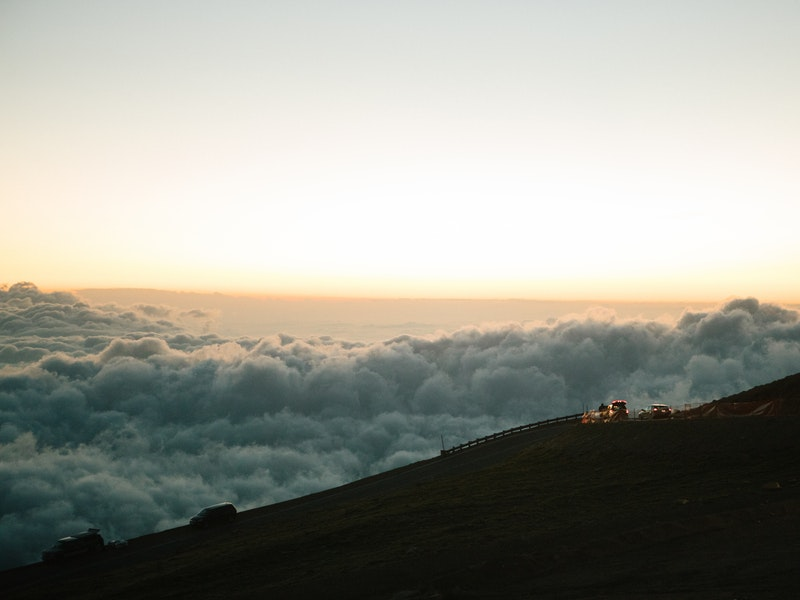
\includegraphics[width=\linewidth]{./result/cloud.jpeg}
        \caption{Original image}
      \end{subfigure}
      \hspace{1cm}
      \begin{subfigure}{.45\textwidth}
        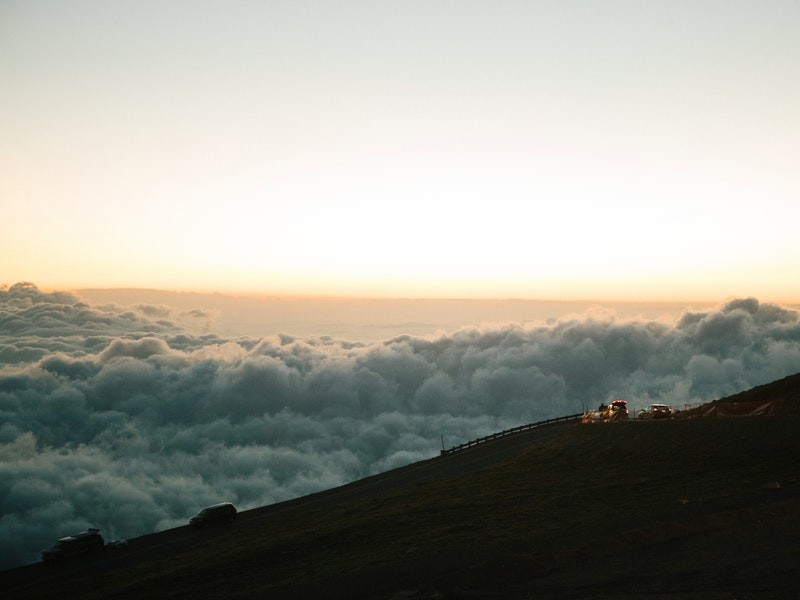
\includegraphics[width=\linewidth]{./result/labwork8-gpu-out.jpg}
        \caption{After conversion}
      \end{subfigure}
    \caption{The output image after convert to HSV and convert back to RGB stays the same as the original input.}
    \end{figure}
\end{itemize}


\end{document}

